%%%%%%%%%%%%%%%%%%%%%%%%%%%%%%%%%%%%%%%%%%%%%%%%%%%%%%%
%
% AUTHOR:lee-shun
%
% DESCRIBTION:第三章--自动驾驶仪控制逻辑
%
%
%%%%%%%%%%%%%%%%%%%%%%%%%%%%%%%%%%%%%%%%%%%%%%%%%%%%%%%

\chapter{无人机动力学模型以及控制器建立}
\label{chap:formation_dynamic_equ}
本章基于无人机编队的领从方法(leader-follower method)建立无人机编队的相对运动方程。再根据飞行力学的相关知识
建立单无人机的运动学模型,之后再介绍单无人机自动驾驶仪的实现逻辑。
\section{无人机动力学模型的建立}
为了与无人机自动驾驶仪的解耦控制方法相匹配,本文将无人机
空间运动分为水平平面运动以及竖直平面运动,并在两个平面内
内分别建立数学模型。由于无人机尺寸小,强度大,飞行包线较小,
并且使用较为成熟的自动驾驶仪,现做如下假设:
\begin{itemize}
    \item 无人机为具有6自由度的三维空间运动刚体。
    \item 忽略地球自转,将地球作为惯性系。
    \item 忽略地球曲率,即所谓的“平板地球假设”。\cite{Wusentang2013}
    \item 由于内环控制率以无人机协调(倾斜)转弯(STT)为基础(详见第\ref{chap:hardware}章),飞机满足无侧滑条件,侧滑角为0;即空速方向与机体系$O_bx_b$在同一竖直平面内。
    \item 由于编队飞行时的区域较小,领机与从机的大气环境以及地球重力场等因素完全一致。
\end{itemize}
本章中涉及的坐标系有:
\begin{enumerate}
    \item 地面坐标系$O_gx_gy_gz_g$:原点$O_g$点选为无人机解锁时的位置,$O_gx_g$轴指向北,$O_gy_g$轴指向东,$O_gz_g$轴符合右手定则,指向下。
    \item 导航坐标系$NED(north-east-down)$:原点选做飞机质心,$N$轴指向北,$E$轴指向东,$D$轴符合右手定则,指向下。
    \item 航迹坐标系$O_kx_ky_kz_k$:原点$O_k$选为无人机质心,$O_kx_k$轴始终与无人机地速方向一致,$O_kz_k$轴位于包含$O_kx_k$轴的竖直平面内,
    $o_ky_k$符合右手定则,指向右。
    \item 机体坐标系$O_bx_by_bz_b$:原点$O_b$选为无人机质心,$O_bx_b$位于无人机的对称平面内,并平行于机身轴线或者机翼的平均气动弦线,指向无人机飞行的前向;$O_bz_b$亦在对称平面之内,
    垂直于$O_bx_b$轴,指向下;$O_by_b$垂直于对称平面,指向右。机体坐标系始终与无人机固连。
    \item 气流坐标系$O_ax_ay_az_a$:气流坐标系又被称作风坐标系或者速度坐标系;原点$O_a$选作无人机质心,$O_ax_a$始终指向无人机的空速方向;$O_az_a$位于无人机对称面之内,
    垂直于$O_ax_a$轴,指向下;$O_ay_a$轴垂直于$O_ax_az_a$平面,指向右。值得注意的是:只有在大气风速$V_{wind}=0$时,航迹系的$O_kx_k$才与气流坐标系的$O_ax_a$重合。
\end{enumerate}
本章中领机与从机的各运动学量以及几何关系分别用上标$l,f$标记,从机期望值以$“des”$上标标记;
运动学量以及几何关系所属坐标系关系则用各个坐标系的字母作为下标标记。
领机、从机在水平以及竖直平面内的几何关系分别在图\ref{fig:c02-2d_level_motion}和图\ref{fig:c02-2d_vert_motion}给出;
\begin{figure}[H]
    \centering
    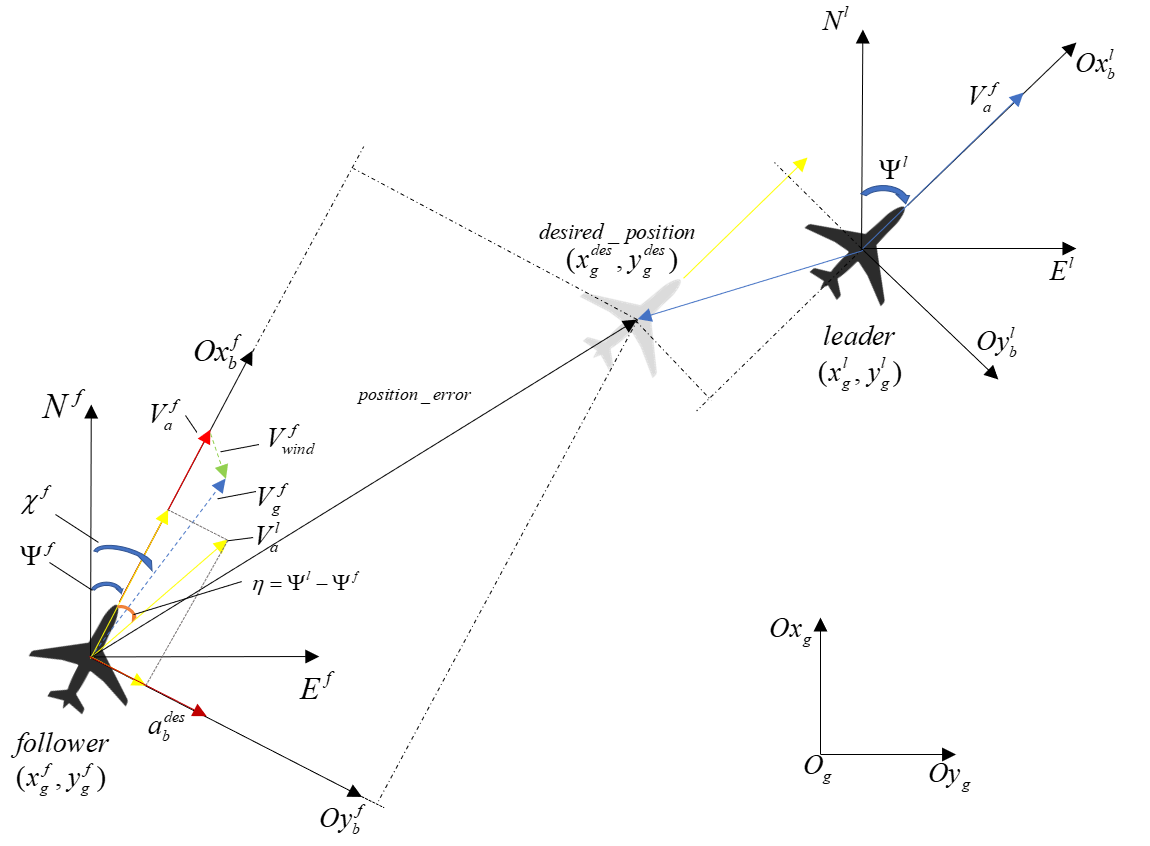
\includegraphics[width=0.75\textwidth]{figures/c2/2d_level_motion.png}
    \caption{水平平面双机编队几何关系}\label{fig:c02-2d_level_motion}
\end{figure}
\begin{figure}[H]
    \centering
    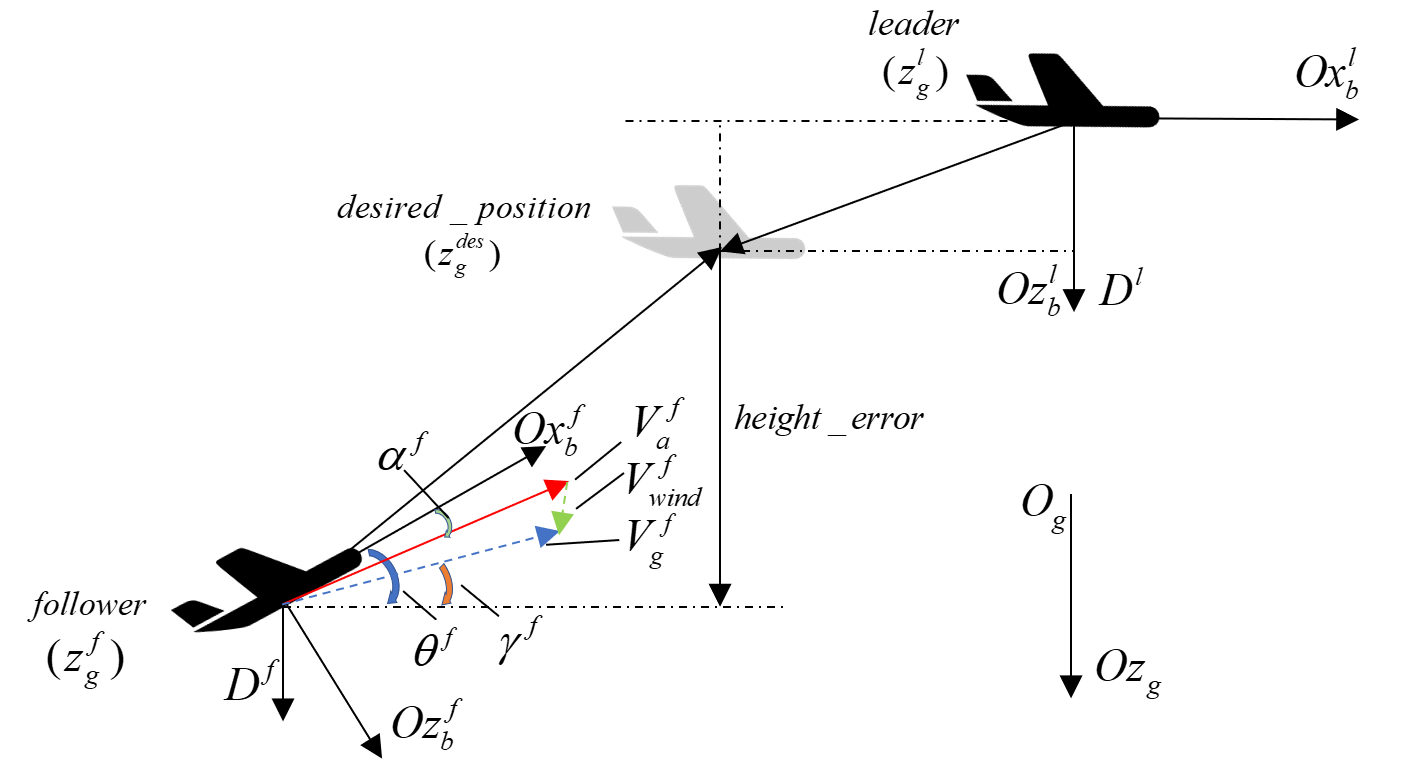
\includegraphics[width=0.75\textwidth]{figures/c2/2d_vert_motion.png}
    \caption{竖直平面双机编队几何关系}\label{fig:c02-2d_vert_motion}
\end{figure}
在图\ref{fig:c02-2d_level_motion}中:
$(x_{g}^l,y_{g}^l),(x_{g}^f,y_{g}^f),(x_{g}^{des},y_{g}^{des})$分别为领机、从机以及从机期望编队位置在地面坐标系$O_gx_gy_g$平面之中的分量;
$\Psi^l,\Psi^f$分别为领机与从机的偏航角(yaw angle);
$\chi^l,\chi^f$分别为领机与从机的航迹偏角(航迹方位角);
$V_a,V_{wind},V_g$分别为领机和从机的空速、风速以及地速向量;
$a_{b}^{des}$是从机产生的、在体轴系下的期望的法向加速度。

在图\ref{fig:c02-2d_vert_motion}中:
$z_{g}^l,,z_{g}^f,z_{g}^{des}$分别为领机、从机以及从机期望编队位置在地面坐标系$O_gz_g$轴上的分量;
$\theta^l,\theta^f$分别为领机与从机的俯仰角(pitch angle);
$\gamma^l,\gamma^f$分别为领机与从机的航迹倾角(航迹倾斜角);
$V_a,V_{wind},V_g$分别为领机和从机的空速、风速以及地速向量;

在图\ref{fig:c02-2d_level_motion}和图\ref{fig:c02-2d_vert_motion}中,由飞机飞行动力学可知,从机与领机三维运动学方程均为:
\begin{equation}
    \left\{
    \begin{array}{l}
        \frac{dx_g}{dt}=V_g\cos\gamma\cos\chi\\
        \frac{dy_g}{dt}=V_g\cos\gamma\sin\chi\\
        \frac{dz_g}{dt}=-V_g\sin\gamma
    \end{array}
    \right .
    \label{fol_motion_eauation}
\end{equation}
现考虑无风情况下,则由图\ref{fig:c02-2d_level_motion}可知,无人机航迹偏角等于航向角,即$\Psi=\chi$;无人机在平衡状态下,迎角很小(本无人机约在2.3°左右),由图\ref{fig:c02-2d_vert_motion}可得$\theta\approx\gamma$。
于是方程组\ref{fol_motion_eauation}可改写为:
\begin{equation}
    \left\{
    \begin{array}{l}
        \frac{dx_g}{dt}=V_g\cos\theta\cos\Psi\\
        \frac{dy_g}{dt}=V_g\cos\theta\sin\Psi\\
        \frac{dz_g}{dt}=-V_g\sin\theta
    \end{array}
    \right .
    \label{fol_motion_eauation1}
\end{equation}
方程组\ref{fol_motion_eauation1}的第1、2两式表示无人机在水平平面内的运动轨迹;第3式表示无人机在竖直平面内的运动轨迹。方程组中,控制的直接输入量为从机的$V_{g}^f,\theta^f,\Psi^f$,再确定飞机的初始运动量之后,可唯一确定领机与从机的
运动规律。

值得注意的是:上述控制量并不能直接由编队控制器产生,但经过理想内环控制器以及无人机动力学模型之后,将产生相应的上述的直接控制量,完整流程将在第\ref{chap:controller_design}章中介绍。
\section{自动驾驶仪控制逻辑}
正如前文所提到的:由于文中编队控制器基于领从方法(leader-follower method),因而领机的飞行完全是由预先给定的一系列航迹点以及自动驾驶仪
所决定的。并且,本文设计的的编队控制器是以现有开源自动驾驶仪PX4的内环为基础;因此,本章将首先介绍控制领机飞行的自动驾驶导航以
及位置模块的实现逻辑,之后将介绍固定翼无人机编队飞行至关重要的基础环节-----自动驾驶仪内环,即姿态内环的实现逻辑。
内环姿态驾驶仪使用的是开源自动驾驶仪PX4。PX4是一个为无人机或者其他无人系统设计的高度模块化、可定制化的、可运行于多种硬件平台的
开源自动驾驶仪软件系统;
PX4为使用集成的开发人员提供了优化的api和sdk。所有模块都是自包含的,可以轻松地针对不同的模块进行交换,而无需修改核心。特性易于部署和重新配置。可以与ROS等机器人操作系统进行数据交互。下图展示了PX4
的软件架构以及各个模块之间的交互关系:
\begin{figure}[H]
    \centering
    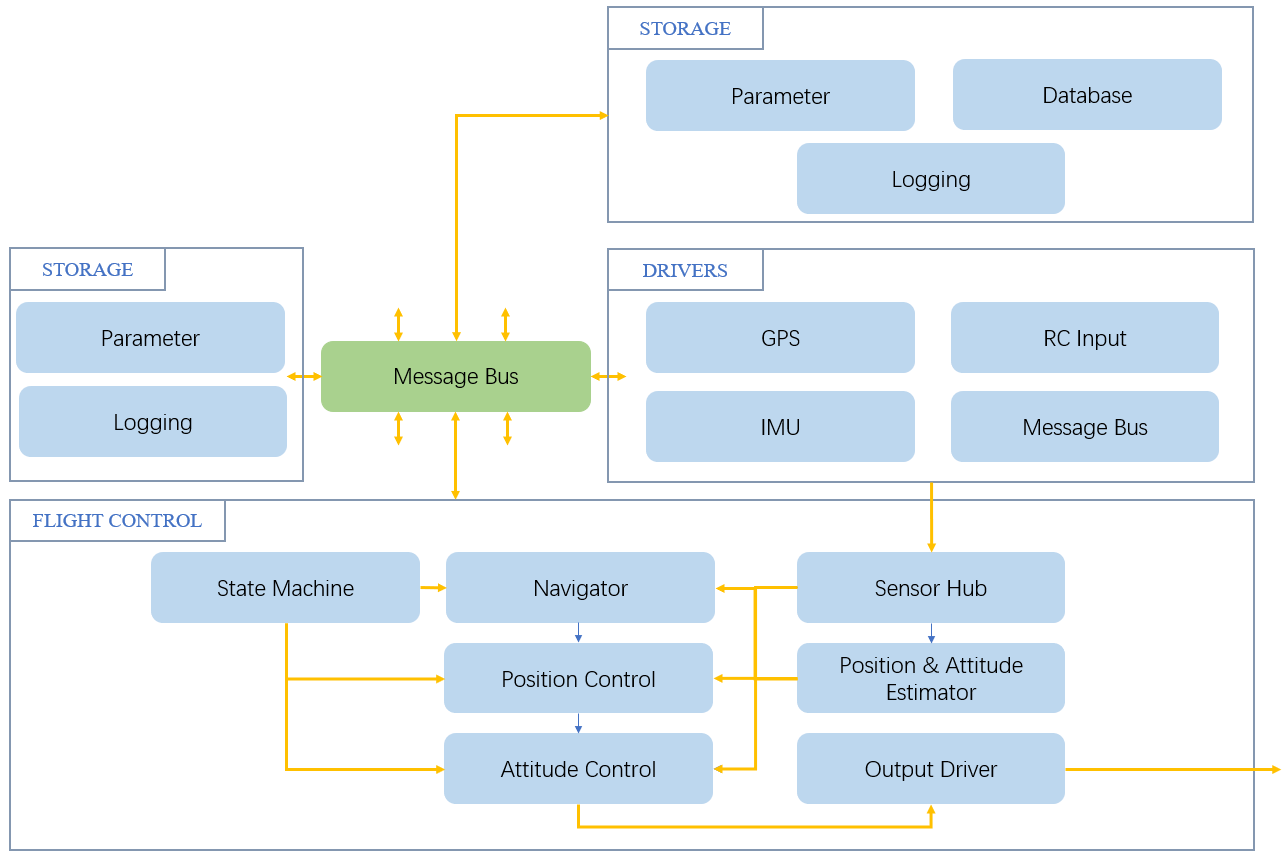
\includegraphics[width=0.8\textwidth]{figures/c4/PX4_archticher.png}
    \caption{PX4软件架构}\label{fig:PX4_archticher.png}
\end{figure}
\subsection{导航以及位置外环实现逻辑}
所谓导航模块(Naigator),其功能是产生相应的期望位置航点。编队中领机按照人为设定的任务策略飞行,导航模块则根据给定的航点以及无人机的位置不断得出当前位置
下的期望航点。导航模块并无控制器参与,本模块是利用既定的飞行策略,产生期望航点,对起飞,降落等特殊飞行环节作出一定得针对性的策略。
本次的编队控制器设计将不涉及导航模块的设计。

位置外环功能是接受来自导航模块的期望位置,再结合无人机的当前位置,按照给定的导航算法,产生姿态内环的所接受的
期望姿态以及期望推力值。位置外环将无人机的运动分为竖直与水平平面的运动,并在上述两个平面内分别设计位置控制器;竖直平面控制器选用
TECS控制器,水平平面选用L1控制器。下面将简要介绍上述两种控制器的控制逻辑:
\subsubsection{TECS控制器控制逻辑}
所谓总能量控制(total energy control)是将无人机的速度以及高度计算得到相应的动能以及势能作为直接控制对象,应用PID控制器对动能与势能的和(total energy)
以及动能与势能的转化(total energy balance)进行控制,计算得到无人机期望俯仰角以及期望推力的控制器。飞机作为一个动力学系统,其机械能来自推力做功的输入,因而总能量控制对应着期望推力;与之对应的俯仰角控制是能量守恒的,
可作为动能向势能(反之亦然)的转化途径,对此种能量转化的控制对应着期望俯仰角。下面简要介绍TECS控制器的计算过程:
\\
无人机的总能量为:
\begin{equation}
    E_T=\frac{1}{2}mV_T^2+mgh
    \label{ET}
\end{equation}
对上式两边微分,可得到总能量变化率:
\begin{equation}
    \dot{E_T}=mV_T\dot{V_T}+mg\dot{h}
    \label{ET_rate}
\end{equation}
由此可得单位总能量变化率:
\begin{equation}
    \dot{E}=\frac{\dot{E}_{T}}{m g V_{T}}=\frac{\dot{V}_{T}}{g}+\frac{\dot{h}}{V_{T}}=\frac{\dot{V}_{T}}{g}+\sin \gamma
    \label{specif_ET_rate}
\end{equation}
更换式\ref{point_dynamaic}第一式形式,可得到:
\begin{equation}
    T-D=m g\left(\frac{\dot{V}_{T}}{g}+\sin \gamma\right)
    \label{point_dynamaic_change}
\end{equation}
由此可得:
\begin{equation}
    \Delta T=m g\left(\frac{\dot{V}_{T}}{g}+sin\gamma\right)
    \label{thrust}
\end{equation}
关于能量转化,定义:
\begin{equation}
    B=m g h-\frac{1}{2} m V_{T}^{2}
\end{equation}
能量转化率为:
\begin{equation}
\dot{B}=sin\gamma-\frac{\dot{V}_{T}}{g}
\end{equation}
这里参照开源自驾仪PX4内部的TECS控制器设计方法,总能量环和能量分配环的控制逻辑框图如下所示:
\begin{figure}[H]
    \centering
    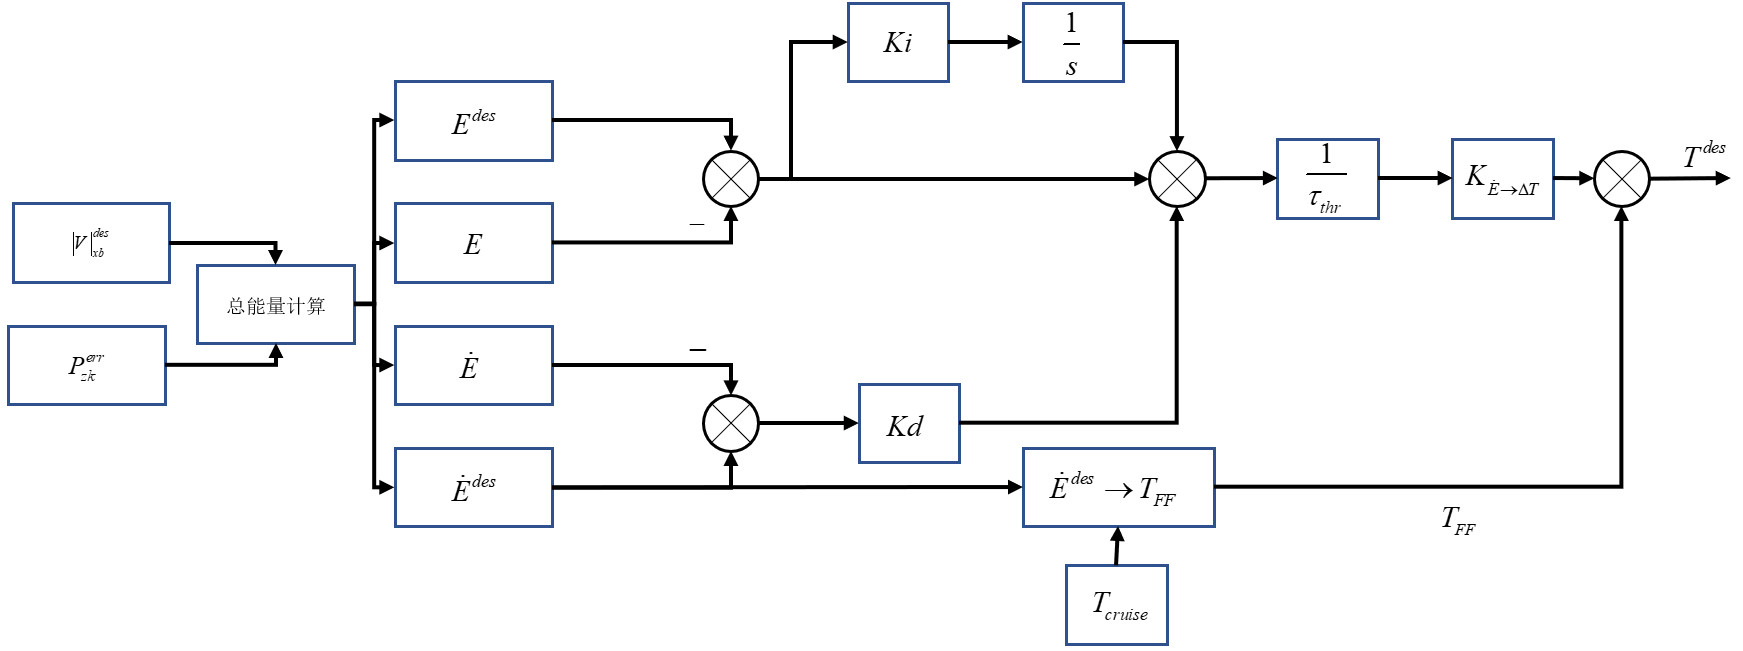
\includegraphics[width=0.9\textwidth]{figures/c3/TECS_throttle.jpg}
    \caption{总能量环}\label{fig:total_energy}
\end{figure}
\begin{figure}[H]
    \centering
    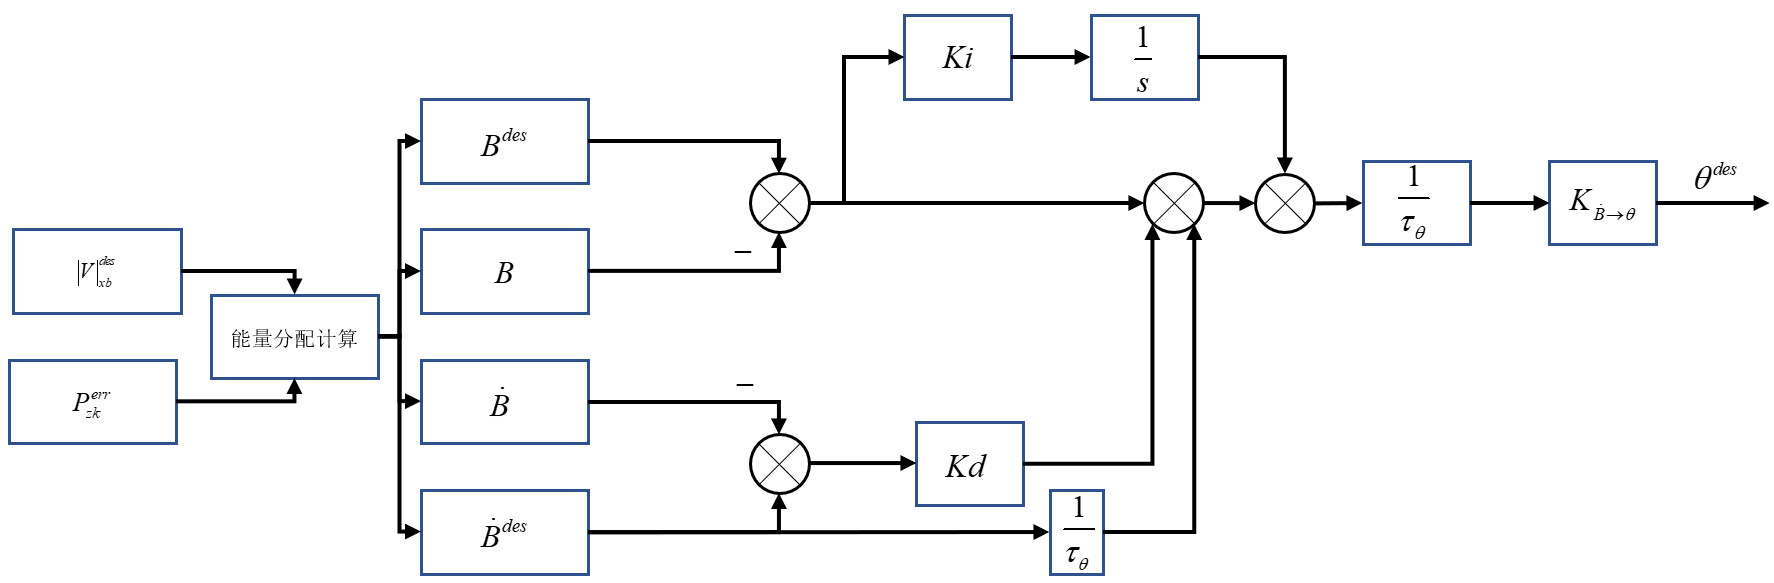
\includegraphics[width=0.9\textwidth]{figures/c3/TECS_pitch.jpg}
    \caption{能量分配环}\label{fig:balance_energy}
\end{figure}
图\ref{fig:total_energy}中,$K_i,K_d,T_{FF},\tau_{thr},K_{\dot{E}\rightarrow\Delta T}$分别为积分项,微分项比例系数,
油门前馈项,油门时间常数以及比例向项系数。
图\ref{fig:balance_energy}中,$K_i,K_d,\tau_{\theta},K_{\dot{B}\rightarrow\Delta \theta}$分别为积分项,微分项比例系数,俯仰角时间常数以及比例向项系数。
\subsubsection{L1控制器实现逻辑}
所谓L1控制器是Sanghyuk Park等人在文献\cite{Park_2004}中提出的一种非线性航迹追踪方法的一种工程实现。Sanghyuk Park在此文中对于此种
控制器的稳定性做了详细的证明,并在不同飞行状态下对此种控制器与传统线性的控制器控制效果做出了完整对比。下面仅作简要介绍:
应用L1控制器分为两步:首先应选取在所控制无人机之前的期望航迹之上的并且距离无人机当前位置为L1距离的参考点,如下图\cite{Park_2004}所示:
\begin{figure}[H]
    \centering
    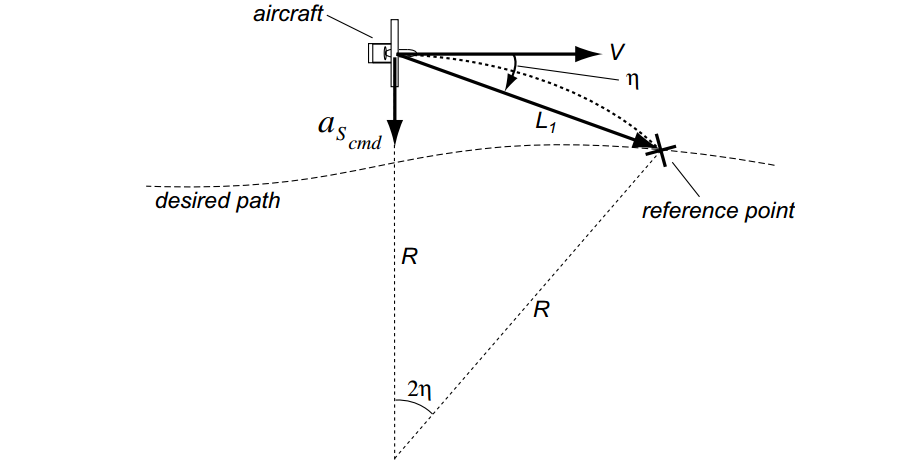
\includegraphics[width=0.75\textwidth]{figures/c3/L1_control}
    \caption{L1控制逻辑图}\label{fig:L1_control}
\end{figure}
之后期望向心加速度$a_{s_{cmd}}$由下式\cite{Park_2004}给出,此式即为L1控制器的导引律。
\begin{equation}
    a_{s_{cmd}}=2\frac{V^2}{L_1}sin\eta
\end{equation}
最终的控制效果为:
\begin{figure}[H]
    \centering
    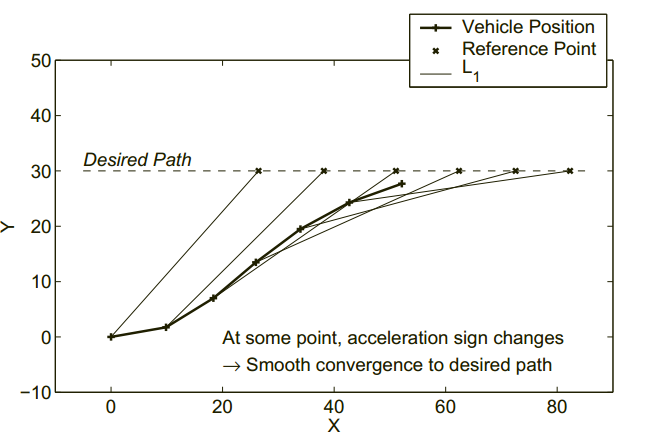
\includegraphics[width=0.75\textwidth]{figures/c3/L1_eff}
    \caption{L1控制器控制效果}\label{fig:c3-L1_eff}
\end{figure}
在做曲线航迹追踪时,按照Sanghyuk Park等人的分析,控制律将近似为PD控制器。
之后,按照实际应用的需要,并参考Paul Riseborough, Brandon Jones 和 Andrew Tridgell等人为另一款开源无人机自动驾驶仪APM的L1
控制器设计,将上述导引律做如下改动:
\begin{enumerate}
    \item 显式表示控制律中的频率以及阻尼。
    \item 显式表示跟踪角度。
    \item 可以使用小于L1长度的盘旋半径。
    \item 修改原始圆形追踪控制律,使用PD控制器使得盘旋时可使用小于L1长度的盘旋半径。
    \item 修改控制逻辑可以分别调整L1控制器的阻尼比以及周期。\label{enu:period}
\end{enumerate}
对于较为关键的第\ref{enu:period}项,最终的$L1$长度选择可由下式表示:
 \begin{equation}
     L_1 = \frac{V}{\pi T_{L1} \xi_{L1}}
\end{equation}
\subsection{姿态内环控制原理}
就总体结构而言,姿态内环的控制方法为为串级PID控制,分为外环角度环,次外环角速度环以及内环角加速度环,其控制框图如下所示:
\begin{figure}[H]
    \centering
    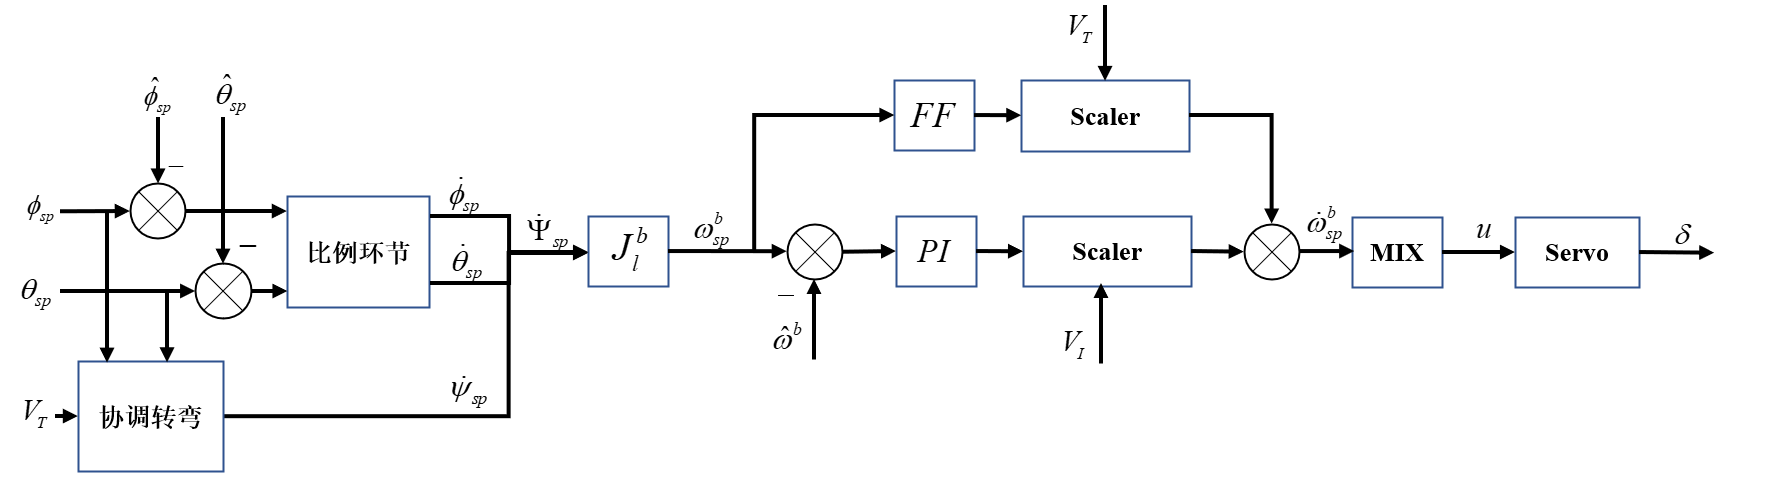
\includegraphics[width=0.90\textwidth]{figures/c3/attitude_inner_loop}
    \caption{姿态内环控制原理框图}\label{c3-attitude_inner_loop}
\end{figure}
其中,$\phi_{sp}$,$\theta_{sp}$,$\psi_{sp}$分别为滚转角、俯仰角以及偏航角期望值;$\dot{\phi}_{sp}$,$\dot{\theta}_{sp}$,$\dot{\psi}_{sp}$
分别为姿态角速度期望值;$\dot{\Psi}_{sp}$为上述期望姿态角速度所组成的三维向量;$J^{b}_l$为无人机由惯性系(地面系)到机体系的转换矩阵;
$V_T$、$V_I$分别为无人机真实空速(true air speed)以及指示空速(indicator air speed);形如“$\hat{\theta}$”的符号为相应
物理量的估计值。

如上图所示,姿态驾驶仪的外环计算期望姿态与估计姿态之间的误差,经过比例控制之后产生角速度期望值。
内环计算速率误差并且利用比例积分控制产生期望的角加速度期望值。

之后,控制面的控制角位置的产生则由期望的角加速度以及无人机系统的先验知识,即控制分配关系所产生。
进一步的,因为在高速下的控制面效率要大于低速下,因而控制器中设计“巡航速度”这一参数来计算空速的影响。

控制器中的前馈增益用来补偿空气动力学阻尼。体轴系下的力矩基本上由控制面以及气动阻尼产生。因此,为了保持滚转角速率为常数,
控制力矩应保持与空气阻尼力矩与大小相等,方向相反,因此此种阻尼可由前馈项计算得出。

内环控制器中的滚转以及俯仰通道的控制器的实现有者相似的结构,均为上述介绍的串级PID控制器,但是在偏航通道上,偏航角度度的期望值是直接由飞机协调转弯条件得出,
以降低在飞机转弯时的衡侧向加速度,具体请参见文献\cite{Fangzhenping2005}
